% !TEX TS-program = xelatex
% !TEX encoding = UTF-8 Unicode

% GSET Summer 2023 - Tennessee Technological University
% Tristan Hill - June 07, 2023
% Turtorial 3 - Ideal Gas Law

\documentclass[12pt]{article}

% Custom Preamble
\usepackage{../../py_tutorials}

% Title and Misc
\newcommand{\MNUM}{3} %Module Number
\newcommand{\MNAME}{Variables and Assignment} %Module Name
\newcommand{\TNAME}{The Ideal Gas Law} %Tutorial Name
\pagestyle{myheadings}
\markright{{\large GSET - Introduction to Programming with Python}}

\begin{document}

\thispagestyle{plain}

\begin{center}
   {\bf \large GSET - Introduction to Programming with Python - Summer 2023} \vspace{5mm}\\
   {\bf \Large \MNAME \hspc -  Tutorial\hspc\MNUM\hspc - \TNAME}\vspace{3mm}\\
   
\end{center}

%\hspace*{3cm}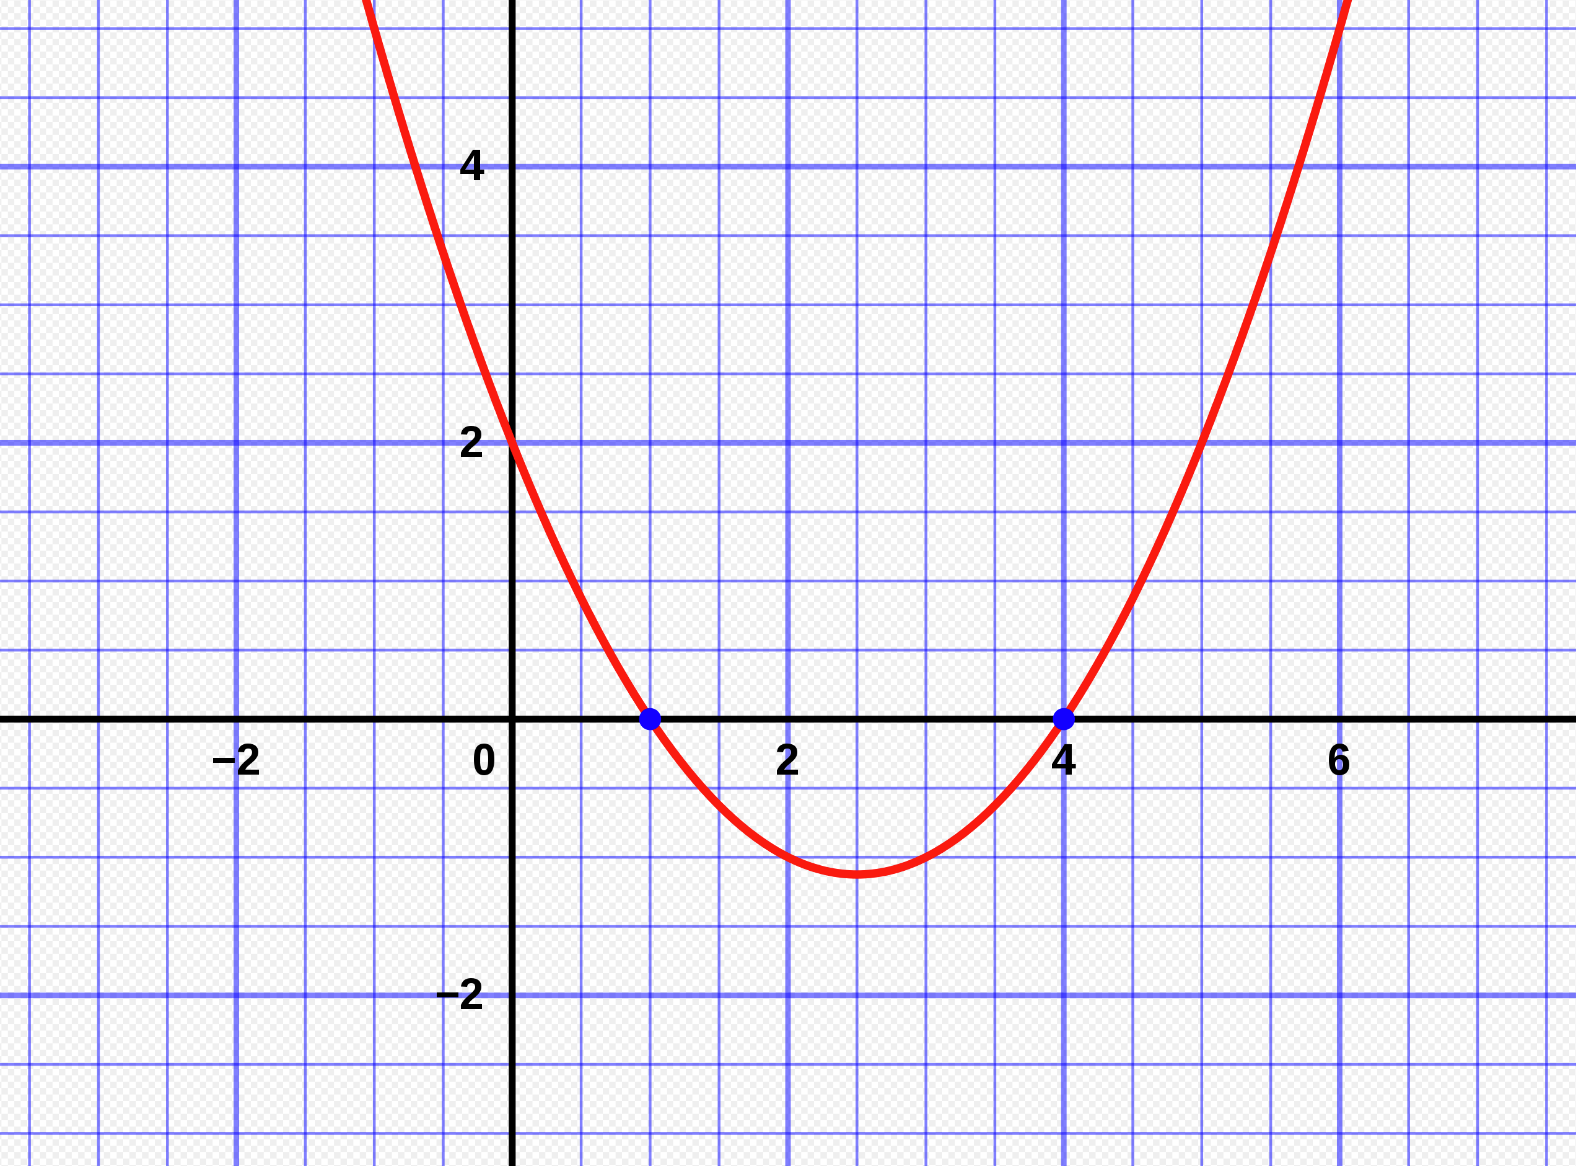
\includegraphics[scale=.15]{quad_equ.png} 

\begin{description}[labelindent=1cm]
	
			\item [\textbf{ \Large Overview}] \textbf{ \Large :}\\
			You will practice sequential calculations and add formatted output to a Python program. The {\it print} function will be used to display formatted strings to the command window. You will complete a basic, but fundamental chemistry calculation. The inputs are typed in your program and the program will output the results to the command window. \\
 	
	\item[\textbf{\underline{System Requirements:}}] \hfill \vspace{0mm}

\begin{itemize}
	\item {\bf Computer}: A computer is required to complete this tutorial. Any OS should work.
	\item {\bf Python:} You can use the online Python compiler ( \href{https://www.online-python.com/online_python_compiler}{Online Python Compiler}  ) or a Python system of your choice.
\end{itemize}

	\item[\textbf{\underline{Background:}}] \hfill \vspace{0mm}
	
	\begin{description}

	 	\item [\textbf{ What is a Mole?}] \textbf{ \Large :}\\   
            The mole is a unit of measurement used in chemistry to express amounts of a chemical substance, defined as the amount of any substance that contains as many elementary entities (e.g., atoms, molecules, ions, electrons) as there are atoms in 12 grams of pure carbon-12. This number is called {\it Avogadro's Constant} and has a value of $6.0221\times10^{23}$. \\
            
      \item [\textbf{ The Ideal Gas Law}] \textbf{ \Large :}\\  
            The following equations describe the behavior of a gas in the form of the temperature, pressure, volume and mass relation. The equation to find the force on the piston is also given. You will use them in your program. \\

             \scalebox{1.3}{$PV=nRT$}   \hspace{15mm}    \scalebox{1.5}{$n=m/M$} \hspace{15mm} \scalebox{1.5}{$P = F/A $} 
      
   \item[\textbf{\underline{Problem Statement:}}] \hfill \vspace{0mm}

	\begin{itemize}

		\item Given: Gas properties, cylinder dimension, and system state
		
		\item Find: Mass and number of moles of gas before and after cylinder position change
		 
	\end{itemize}      

            \newpage                     
            where,\\
            
            \begin{multicols}{2}
            
            \begin{tabular}{lll}
            x &position &($m$)   \\
            F &force    &($N$)   \\
            V &volume   &($m^3$) \\        
            n &number of moles &($mols$) \\   
            m & mass of gas&($kg$)      \\ 
            \\
            A=100 &area     &($cm^2$)  \\
            P=300 &pressure &($kPa$) \\ 
            T=325 & temperature &($K$) \\\\ 
            M=28.97 & molecular mass of air &($\frac{g}{mol}$)       \\\\ 
            R=8.314 & ideal gas constant &($\frac{Pa\hspace{1mm}m^3}{mol\hspace{1mm}K}$)\\ 
            \end{tabular}\\

            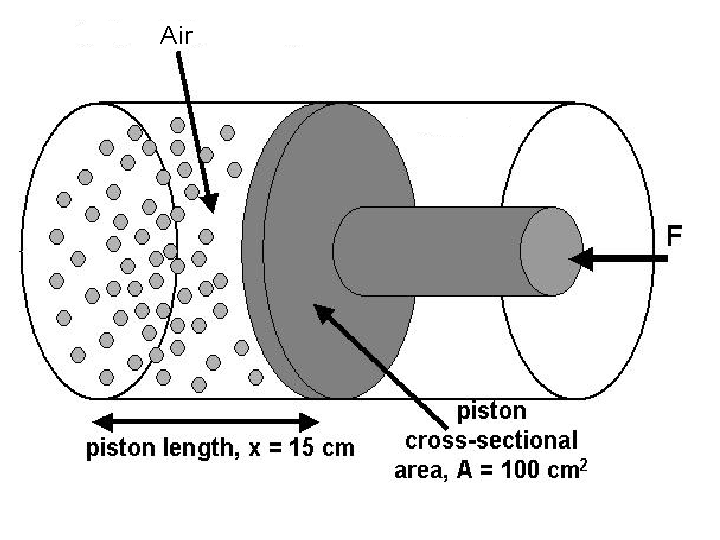
\includegraphics[scale=.30]{ideal_gas_law_fig1.png} \\    
            \end{multicols}
               1($kPa$)=1000($Pa$)\\
               1($Pa$)=1($\frac{N}{m^2}$)

	\end{description}



\item[\textbf{\underline{Program Minimum Requirements:}}] \hfill \vspace{0mm}

The program should accomplish the following tasks. 


\begin{enumerate}
            \item
            {\bf R}, {\bf M}, {\bf T}, {\bf P}, and {\bf A}, are constants. {\it Hardcode} these in your program. \\
            \item
            Consider the piston at position  {\bf x=15 cm}. Calculate the force, {\bf F} required to hold the piston at the current position..\\	
            \item
            Calculate the remaing quantities {\bf V}, {\bf n}, and {\bf m}.\\ 
            \item
            Output the 4 results to the command window in the {\it base S.I. units}. \\
            \item
            Consider the piston has moved to {\bf x=10 cm} and the temperature, T stays constant. Calculate and output the quantities that have changed. Do not output the quantities that have \underline{not} changed.\\\\  
\end{enumerate}	 

	Optional Advanced Features:
\begin{itemize}
	\item The inputs $T$ and $A$ should be read from the user input during program execution
		
    
\end{itemize}	
\newpage

\item[\textbf{\underline{Example Code:}}] \hfill \vspace{0mm}

	%\begin{minted}{cpp}
	\begin{lstlisting}

# Variables and Assignment - GSET - Summer 2023 
	

	
	\end{lstlisting}
	%\end{minted}
		


	\item[\textbf{\underline{Part 3 - Testing:}}] \hfill \vspace{0mm}
	\begin{enumerate}
	
		\item Complete the Python code to the solve the problem described. \\\\
		
		\item Test your code with different inputs. Is the answer correct? How do you know? Are there certain inputs that do not work? \\\\
		
		\item Save your code with the download button or use copy and paste. You can view and edit the code in any text editor. Also, save a copy of the program output for your tutorial summary. \\\\

	\end{enumerate}

\newpage
\item[\textbf{\underline{Solution Code:}}] \hfill \vspace{0mm}

\begin{lstlisting}

COMING SOON
	
\end{lstlisting}

\item[\textbf{\underline{Tutorial Summary:}}] \hfill \vspace{3mm}\\ 
Write a brief summary of what you accomplished and what you struggled with the most. 

Include the following items in the summary:
\begin{itemize}

\item a copy of the output of your program
\item a description of what the program does and how to use it

\end{itemize}


\item[\textbf{\underline{Submission on Teams:}}] \hfill \vspace{3mm}\\ 
Use the appropriate assignment folder on ilearn to submit your program and summary. Submit the following items with your TNTech username in the filenames as shown below. \vspace{0mm}\\

\underline{Files for Tutorial 3 (TNTech Username : twhill21)}

\begin{itemize}

\item Tutorial Summary: \textbf{ twhill21\_summary3.txt}

\item Python Source Code: \textbf{ twhill21\_tutorial3.py}

\end{itemize}


\item[\textbf{\underline{Tutorial Complete:}}] \hfill \vspace{3mm}\\ 
	Congratulations, after completing {\it Tutorial 3 - The Ideal Gas Law}, you have begun learning to program in Python! You are now ready to start learning about more complex data structures and program flow. \\

\end{description}
\end{document}

